\documentclass[aps,prb,reprint]{revtex4-2}
\usepackage{amsmath,amssymb}
\usepackage{pgfplots}
\pgfplotsset{compat=1.18}
% Make every plot inherit the document's serif face.  Without this the axis
% text falls back to the sans-serif default and the figure looks pasted in
% rather than typeset with the paper.
\pgfplotsset{
  every axis/.append style={font=\rmfamily},
  tick label style={font=\footnotesize\rmfamily},
  label style={font=\small\rmfamily},
  legend style={font=\scriptsize\rmfamily},
}
\definecolor{gmeC0}{HTML}{1F77B4}
\definecolor{gmeC1}{HTML}{FF7F0E}
\definecolor{gmeC2}{HTML}{2CA02C}
\definecolor{gmeC3}{HTML}{D62728}
\definecolor{gmeC4}{HTML}{9467BD}
\definecolor{gmeC5}{HTML}{8C564B}
\definecolor{gmeC6}{HTML}{E377C2}
\definecolor{gmeC7}{HTML}{17BECF}
\begin{document}
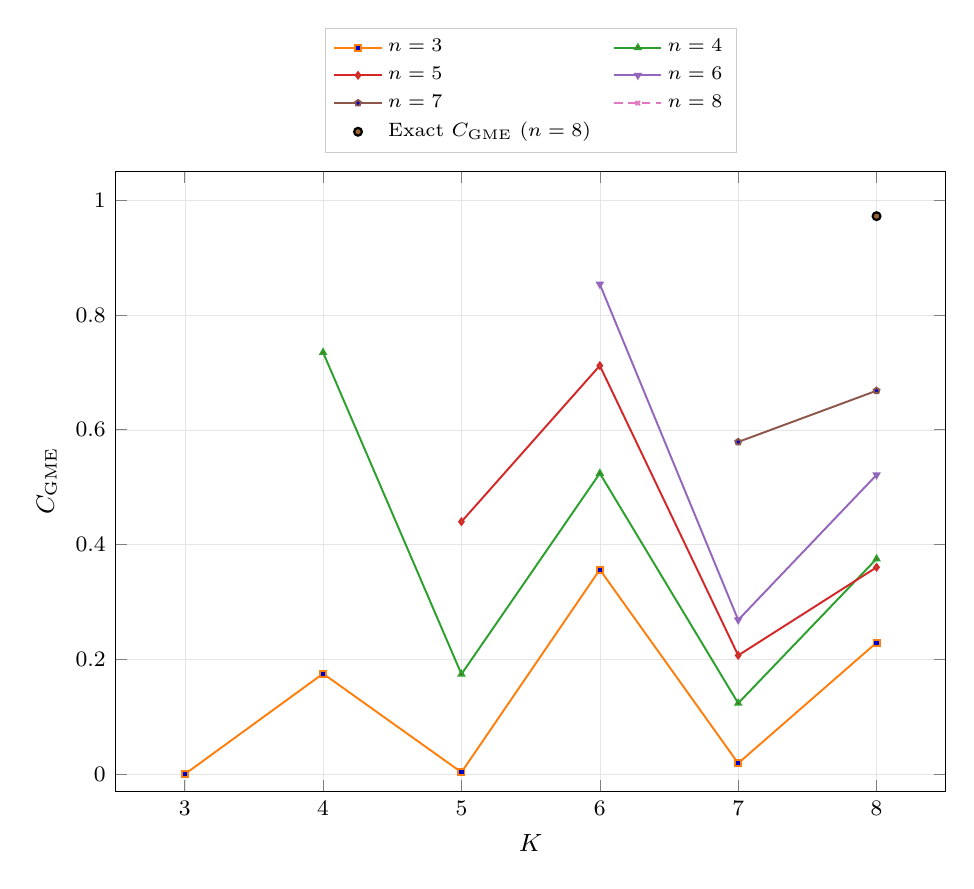
\begin{tikzpicture}
  \begin{axis}[
    width=\columnwidth,
    height=0.78\columnwidth,
    xlabel={$K$},
    ylabel={$C_{\mathrm{GME}}$},
    grid=both,
    grid style={line width=.1pt, draw=gray!20},
    tick label style={font=\footnotesize\rmfamily, /pgf/number format/fixed},
    label style={font=\small\rmfamily},
    scaled ticks=false,
    legend style={font=\scriptsize\rmfamily, draw=gray!40, at={(0.5,1.03)}, anchor=south, /tikz/every even column/.append style={column sep=6pt}},
    legend cell align={left},
    legend columns=2,
    ymin=-0.03,
    ymax=1.05,
  ]
    \addplot+[color=gmeC1, mark=square*, mark size=1.1pt, line width=0.7pt] coordinates {
        (3,0) (4,0.175239) (5,0.003431) (6,0.356408)
        (7,0.019139) (8,0.229253)
    };
    \addlegendentry{$n=3$}
    \addplot+[color=gmeC2, mark=triangle*, mark size=1.1pt, line width=0.7pt] coordinates {
        (4,0.734639) (5,0.174351) (6,0.524127) (7,0.12367)
        (8,0.375187)
    };
    \addlegendentry{$n=4$}
    \addplot+[color=gmeC3, mark=diamond*, mark size=1.1pt, line width=0.7pt] coordinates {
        (5,0.439793) (6,0.711589) (7,0.206995) (8,0.360429)
    };
    \addlegendentry{$n=5$}
    \addplot+[color=gmeC4, mark=triangle*, mark size=1.1pt, mark options={rotate=180}, line width=0.7pt] coordinates {
        (6,0.85338) (7,0.268687) (8,0.521341)
    };
    \addlegendentry{$n=6$}
    \addplot+[color=gmeC5, mark=pentagon*, mark size=1.1pt, line width=0.7pt] coordinates {
        (7,0.578698) (8,0.667932)
    };
    \addlegendentry{$n=7$}
    \addplot+[color=gmeC6, mark=x, mark size=1.1pt, line width=0.7pt] coordinates {
        (8,0.97189)
    };
    \addlegendentry{$n=8$}
    \addplot+[color=black, dashed, mark=*, mark size=1.4pt, only marks, line width=0.8pt] coordinates {
        (8,0.97189)
    };
    \addlegendentry{Exact $C_{\mathrm{GME}}$ ($n=8$)}
  \end{axis}
\end{tikzpicture}

\end{document}
